\chapter{Petites oscillations}

\section{Oscillations lin\'eaires libres}\label{PAR:21}

Les \emph{petites oscillations} sont celles faites par un syst\`eme au voisinage de sa position d'\'equilibre stable et nous étudions ici le cas le plus simple, celui où il n'y a qu'un seul degr\'e de libert\'e. Un \'equilibre stable intervient quand l'\'energie potentielle $U(q)$ est minimale. D\'efinissons que $U$ soit minimale en $q = q_{0}$. L'\'equation (\ref{EQ:5_4}) montre qu'un \'ecart par rapport \`a la position $q_{0}$ engendre une force \'egale \`a $-\frac{\mathrm{d}U}{\mathrm{d}q}$ qui ram\`ene le syst\`eme \`a sa position d'\'equilibre stable. R\'ealisons un d\'eveloppement de Taylor de $U(q)$ jusqu'au second ordre :
\benn
	U(q) = U(q_{0}) + U'(q_{0})(q - q_{0}) + \dfrac{U''(q_{0})}{2}(q - q_{0})^{2} \Rightarrow U(q) - U(q_{0}) = \dfrac{k}{2}(q - q_{0})^{2}
\eenn
car $U'(q_{0}) = 0$ puisque $q_{0}$ est la position d'\'equilibre et nous avons pos\'e $k = U''(q_{0})$. En d\'efinissant :
\be
	x = q - q_{0} \label{EQ:21_1}
\ee
qui repr\'esente l'\'ecart par rapport \`a la position d'\'equilibre, nous avons, en posant $U(q_{0}) = 0$ :
\be
	U(x) = \dfrac{kx^{2}}{2} \label{EQ:21_2}
\ee
Au regard des relations (\ref{EQ:4_1}) et (\ref{EQ:5_5}), l'\'energie cin\'etique pour une particule et dans le cas d'un unique degr\'e de libert\'e, s'\'ecrit $T = \frac{1}{2}a(q)\dot{q}^{2}$. Or dans le cadre des petites oscillations, $x \approx q$. De la m\^eme mani\`ere, $a(q) \approx q(a_{0})$, quantit\'e qui peut s'identifier \`a la masse de la particule si $x$ est une coordonn\'ee cart\'esienne. L'\'energie cin\'etique peut donc se formuler comme $T = \frac{1}{2}m\dot{x}^{2}$. Par cons\'equent, la fonction de Lagrange pour un syst\`eme r\'ealisant de petites oscillations, d\'enomm\'e aussi \emph{oscillateur lin\'eaire} est :
\be
	L = \dfrac{m\dot{x}^{2}}{2} - \dfrac{kx^{2}}{2} \label{EQ:21_3}
\ee
Dans notre cas \'epur\'e, l'\'equation du mouvement s'obtient \`a partir de la relation (\ref{EQ:5_2}) :
\be
	\dfrac{\mathrm{d}}{\mathrm{dt}}\left(\dfrac{\partial L}{\partial \dot{x}}\right) = \dfrac{\partial L}{\partial x} \Leftrightarrow \dfrac{\mathrm{d}m\dot{x}}{\mathrm{dt}} = -kx \Leftrightarrow m\ddot{x} + kx = 0 \label{EQ:21_4}
\ee
\'Equation qui peut \'egalement s'\'ecrire :
\be
	\ddot{x} + \omega^{2}x = 0 \label{EQ:21_5}
\ee
en posant la quantit\'e :
\be
	\omega = \sqrt{\dfrac{k}{m}} \label{EQ:21_6}
\ee
qui est appel\'ee \emph{fr\'equence angulaire}. La quantit\'e $\omega$ ne d\'epend pas des conditions initiales du mouvement mais uniquement des propri\'et\'es m\'ecaniques du syst\`eme, c'est une constante fondamentale des oscillations. Ceci n'est valable que dans le cas qui nous concerne, celui des petites oscillations, ou encore quand $U \propto x^{2}$. Pour les cas g\'en\'eraux, nous pouvons nous reporter \`a l'\'equation (\ref{EQ:11_EX2A_1}) qui d\'efinit la p\'eriode d'oscillations $T$ pour $U = A\lvert x^{n} \rvert$, sachant que $\omega = 2\pi/T$.

L'\'equation (\ref{EQ:21_5} admet deux solutions ind\'ependantes en $\cos(\omega t)$ et en $\sin(\omega t)$. Donc la solution g\'en\'erale s'\'ecrit :
\be
	x = c_{1}\cos(\omega t) + c_{2}\sin(\omega t) \label{EQ:21_7}
\ee
ou encore :
\be
	x = a\cos(\omega t + \alpha) \label{EQ:21_8}
\ee
o\`u $a$ est l'\emph{amplitude} et $\alpha$ la valeur initiale de la \emph{phase}, qui d\'epend de l'origine prise pour $t$.Comme $\cos(\omega t + \alpha) = \cos(\omega t)\cos\alpha - \sin(\omega t)\sin\alpha$, alors nous pouvons en d\'eduire, \`a partir de la relation (\ref{EQ:21_7}), $c_{1} = a\cos\alpha$ et $c_{2} = -a\sin\alpha$. De plus :
\be
	\begin{cases}
		c_{1}^{2} + c_{2}^{2} = a^{2}(\cos^{2}\alpha + \sin^{2}\alpha) \Rightarrow a = \sqrt{c_{1}^{2} + c_{2}^{2}} \\
		\dfrac{\sin\alpha}{\cos\alpha} = \tan\alpha = -\dfrac{c_{2}}{c_{1}} \label{EQ:21_9}
	\end{cases}
\ee
L'\'energie totale du syst\`eme vaut, en y ajoutant la formule (\ref{EQ:21_8}) :
\bea
	E & = & T + U = \dfrac{m\dot{x}^{2}}{2} + \dfrac{kx^{2}}{2} = \dfrac{m}{2}(\dot{x}^{2} + \omega^{2}x^{2}) \nonumber \\
	& = & \dfrac{m}{2}(a^{2}\omega^{2}\sin^{2}(\omega t + \alpha) + a^{2}\omega^{2}\cos^{2}(\omega t + \alpha)) = \dfrac{m\omega^{2}a^{2}}{2} \label{EQ:21_10}
\eea
Il est souvent ais\'e de passer dans le domaine complexe pour simplifier les op\'erations math\'ematiques et de consid\'erer la solution (\ref{EQ:21_8}) comme :
\be
	x = \Re{\{Ae^{i\omega t}\}} \label{EQ:21_11}
\ee
avec l'\emph{amplitude complexe} s'exprimant comme :
\be
	A = ae^{i\alpha} \label{EQ:21_12}
\ee
dont le module est l'amplitude ordinaire et l'argument la phase initiale.

\section{Oscillations forc\'ees}\label{PAR:22}

Les \emph{oscillations forc\'ees} sont les oscillations d'un syst\`eme soumis \`a un champ ext\'erieur variable. En restant dans l'hypoth\`ese des petites oscillations, cela implique que le champ ext\'erieur est suffisamment faible pour provoquer des d\'eplacements faibles \'egalement. De plus, ici, nous restons dans le cadre d'un unique degr\'e de libert\'e.

\subsection{Cas g\'en\'eral}

L'\'energie potentielle totale du syst\`eme s'\'ecrit avec deux termes, \`a savoir l'\'energie potentielle propre en $\frac{1}{2}kx^{2}$ et celle due \`a l'action ext\'erieur $U_{e}(x,t)$. Au premire ordre, cette derni\`ere s'\'ecrit :
\benn
	U_{e}(x,t) = U_{e}(0,t) + x\left(\dfrac{\partial U_{e}}{\partial x}\right)(0,t)
\eenn
o\`u $U_{e}(0,t)$ est une fonction ne d\'ependant que du temps et de facto, elle est le r\'esultat d'une d\'eriv\'ee totale par rapport au temps. Dans cette partie est n\'eglig\'ee dans l'\'equation de Lagrange, voir (\ref{EQ:2_8}). De plus, la formule (\ref{EQ:5_8}) permet de d\'eduire que $-\frac{\partial U_{e}}{\partial x}$ est la force ext\'erieure qui s'exerce sur le syst\`eme. Elle est fonction du temps et nous la d\'esignons $F(t)$. Par cons\'equent, $U_{e}(x,t) = -xF(t)$ et la fonction de Lagrange peut se formuler ainsi :
\be
	L = \dfrac{m}{2}\dot{x}^{2} - \left(\frac{k}{2}x^{2} - xF(t)\right) \label{EQ:22_1}
\ee
L'\'equation du mouvement provenant de la formule (\ref{EQ:5_2}) permet d'en d\'eduite :
\bea
	\dfrac{\mathrm{d}}{\mathrm{dt}}\left(\dfrac{\partial L}{\partial \dot{x}}\right) & = & \dfrac{\partial L}{\partial x} \Leftrightarrow \dfrac{\mathrm{d}m\dot{x}}{\mathrm{dt}} = -kx + F(t) + x\dfrac{\partial F(t)}{\partial x} \nonumber \\
	& \Leftrightarrow & m\ddot{x} + kx = F(t) \Leftrightarrow \ddot{x} + \omega^{2}x = \dfrac{F(t)}{m} \label{EQ:22_2}
\eea
avec $\omega = \sqrt{\frac{k}{m}}$ la fr\'equence des oscillations. L'\'equation (\ref{EQ:22_2}) est une \'equation diff\'erentielle du second ordre avec des c{\oe}fficients constants et un second membre. La solution g\'en\'erale est de la forme $x = x_{0} + x_{1}$ telle que :
\begin{itemize}
	\item $x_{0}$ est la solution g\'en\'erale de l'\'equation sans second membre qui repr\'esente les oscillations libres d\'etermin\'ee aux \'equations (\ref{EQ:21_7}) et (\ref{EQ:21_8})
	\item $x_{1}$ est une int\'egrale particuli\`ere de l'\'equation avec le second membre
\end{itemize}

\subsection{Cas particulier d'une force ext\'erieure p\'eriodique}

Consid\'erons que la force ext\'erieure s'exprime telle que :
\be
	F(t) = f\cos(\gamma t + \beta) \label{EQ:22_3}
\ee
Pour cette hypoth\`ese, l'int\'egrale particuli\`ere de l'\'equation (\ref{EQ:22_2}) peut \^etre $x_{1} = b\cos(\gamma t + \beta)$, ce qui nous donne :
\bea
	& & -b\gamma^{2}\cos(\gamma t + \beta) + \omega^{2}b\cos(\gamma t + \beta) = \dfrac{f}{m}\cos(\gamma t + \beta) \Leftrightarrow b(\omega^{2} - \gamma^{2}) = \dfrac{f}{m} \nonumber \\
	& \Leftrightarrow & b = \dfrac{f}{m(\omega^{2} - \gamma^{2})} \nonumber
\eea
Le mouvement se compose donc en ajoutant la solution g\'en\'erale (\ref{EQ:21_8}) :
\be
	x = a\cos(\omega t + \alpha) + \frac{f}{m(\omega^{2} - \gamma^{2})}\cos(\gamma t + \beta) \label{EQ:22_4}
\ee
o\`u les quantit\'es $a$ et $\alpha$ sont d\'eduites des conditions initiales. Le mouvement est ainsi compos\'e de la somme de deux oscillations, la premi\`ere avec la fr\'equence propre du syst\`eme et la seconde avec la fr\'equence de la force ext\'erieure. La formule (\ref{EQ:22_4}) est ind\'etermin\'ee dans le cas o\`u $\omega = \gamma$, il y a alors \emph{r\'esonnance}.

\subsection{Solution r\'eelle lors de la r\'esonnance avec une force ext\'erieure}

Partons de la formule (\ref{EQ:22_4}) pour la reformuler ainsi :
\benn
	x = a\cos(\omega t + \alpha) + \frac{f}{m(\omega^{2} - \gamma^{2})}(\cos(\gamma t + \beta) - \cos(\omega t + \beta))
\eenn
Ainsi lorsque $\gamma \rightarrow \omega$, alors nous avons une ind\'etermination de type $0/0$ pour le second terme. Appliquons alors la r\`egle de L'Hospital\footnote{Si $f$ et $g$ sont deux fonctions d\'efinies sur $[a;b[$, d\'erivables en $a$ et telles que $f(a) = g(a) = 0$ et $g'(a) \neq 0$ alors $\lim_{x \rightarrow a^{+}}\dfrac{f(x)}{g(x)} = \dfrac{f'(a)}{g'(a)}$} avec :
\benn
	\begin{cases}
		f : \omega \mapsto \cos(\gamma t + \beta) - \cos(\omega t + \beta) \\
		g : \omega \mapsto w^{2} - \gamma^{2}
	\end{cases}
\eenn
Cela nous donne :
\benn
	\lim_{\gamma \rightarrow \omega}\dfrac{f(\gamma)}{g(\gamma)} = \dfrac{f'(\gamma = \omega)}{g'(\gamma = \omega)} = \dfrac{-t\sin(\omega t + \beta)}{-2\omega}
\eenn
et nous permet d'\'ecrire :
\be
	x = a\cos(\omega t + \alpha) + \frac{f}{2m\omega}t\sin(\omega t + \beta) \label{EQ:22_5}
\ee
Dans le cas de la r\'esonnance, l'amplitude augmente lin\'eairement avec le temps tant que nous restons dans le cadre des petites oscillations.

\subsection{Solution complexe lors de la r\'esonnance avec une force ext\'erieure}

Au voisinage de la r\'esonnance, d\'efinissons la fr\'equence $\gamma = \omega + \epsilon$ avec $\epsilon$ petit devant $\omega$. Dans le domaine complexe, il est possible de g\'en\'eraliser l'expression (\ref{EQ:22_4}) telle que :
\be
	x = Ae^{i\omega t} + Be^{i(\omega + \epsilon)t} = \left(A + Be^{i\epsilon t}\right)e^{i\omega t} \label{EQ:22_6}
\ee
Comme $\epsilon \ll \omega$, l'expression $A + Be^{i\epsilon t}$ varie peu lors d'une p\'eriode $2pi/\omega$. Au voisinage de la r\'esonnance, le mouvement se constitue de petites oscillations \`a amplitude variable. L'amplitude reste une grandeure r\'eelle aussi nous d\'efinissons $C = \lvert A + Be^{i\epsilon t} \lvert$. La relation (\ref{EQ:21_12}) permet d'\'ecrire $A = ae^{i\alpha}$ et $B = be^{i\beta}$, et ainsi l'amplitude $C$ devient :
\bea
	C & = & \lvert ae^{i\alpha} + be^{i(\epsilon t + \beta)} \rvert \nonumber \\
	\Leftrightarrow C^{2} & = & \lvert ae^{i\alpha} \rvert^{2} + \lvert be^{i(\epsilon t + \beta)} \rvert^{2} + 2\lvert ae^{i\alpha} \rvert \cdot \lvert be^{i(\epsilon t + \beta)} \rvert \cos(\epsilon t + \beta - \alpha) \nonumber \\
	C^{2} & = & a^{2} + b^{2} + 2ab\cos(\epsilon t + \beta - \alpha) \label{EQ:22_7}
\eea
Les valeurs extremum de $C$ sont :
\begin{itemize}
	\item $C_{max}^{2} = a^{2} + b^{2} + 2ab \Rightarrow C_{max} = a + b$
	\item $C_{min}^{2} = a^{2} + b^{2} - 2ab \Rightarrow C_{min} = \lvert a - b \rvert$
\end{itemize}
Par cons\'equent, l'amplitude $C$ oscille p\'eriodiquement entre les deux valeurs pr\'ec\'edentes avec une fr\'equence $\epsilon$, ph\'enom\`ene appel\'e \emph{battements}.

Ensuite, nous pouvons remarquer que l'\'equation (\ref{EQ:22_2}) peut s\'ecrire :
\bea
	\ddot{x} + i\omega\dot{x} - i\omega\dot{x} - i\omega\cdot i\omega x & = & \dfrac{F(t)}{m} \Leftrightarrow \dfrac{\mathrm{d}}{\mathrm{dt}}(\dot{x} + i\omega x) - i\omega(\dot{x} + i\omega x) = \dfrac{F(t)}{m} \nonumber \\
	\Rightarrow \dfrac{\mathrm{d}\xi}{\mathrm{dt}} - i\omega\xi = \dfrac{F(t)}{m} \label{EQ:22_8}
\eea
en d\'efinissant la quantit\'e $\xi$ telle que :
\be
	\xi = \dot{x} + i\omega x \label{EQ:22_9}
\ee
L'\'equation (\ref{EQ:22_8}) n'est plus du second ordre. Sa solution g\'en\'erale sans second membre peut d'\'ecrire comme $\xi_{0}e^{i\omega t}$ avec $\xi_{0}$ une constante d\'ependant des conditions initialies et \'egale \`a $\xi(t=0)$. Cherchons d\'esormais un int\'egrale particuli\`ere de la forme $A(t)e^{i\omega t}$ pour l'\'equation avec second membre. En ins\'erant cette solution particuli\`ere dans l'\'equation (\ref{EQ:22_8}) :
\bea
	\dot{A}(t)e^{i\omega t} + i\omega A(t)e^{i\omega t} - i\omega e^{i\omega t} & = & \dfrac{F(t)}{m} \Leftrightarrow \dot{A}(t) = \dfrac{1}{m}F(t)e^{-i\omega t} \nonumber \\
	\Rightarrow \xi(t) & = & e^{i\omega t}\left(\xi_{0} + \dfrac{1}{m}\int{F(t)e^{-i\omega t}\mathrm{dt}}\right) \label{EQ:22_10}
\eea
Ainsi la quantit\'e $x(t)$ est donn\'ee par la partie imaginaire de $\xi(t)$ donn\'ee par la relation (\ref{EQ:22_10}), divis\'ee par $\omega$.

Dans le cas d'oscillations forc\'ees, l'\'energie totale du syst\`eme ne se conservent \'evidemmment pas. L'\'energie totale transmise au syst\`eme par la force ext\'erieure sachant que cette \'energie est nulle initialement, peut se calculer \`a partir de la relation (\ref{EQ:22_10}) :
\be
	E = T + U = \dfrac{m}{2}\dot{x}^{2} + kx^{2} = \dfrac{m}{2}(\dot{x}^{2} + \omega^{2}x^{2}) = \dfrac{m}{2}(\dot{x} + i\omega x)(\dot{x} - i\omega x) = \dfrac{m}{2}\lvert \xi \rvert^{2} \label{EQ:22_11}
\ee
sachant que les quantit\'es $x$ et $\xi$ incluent d\'ej\`a les cons\'equences de la force ext\'erieure $F$ dans leur expression respective. En supposant $\xi(-\infty) = 0$ et parce que $\lvert e^{i\omega t} \rvert = 1$ par d\'efinition, l'\'energie transmise totale vaut en reprenant les relations (\ref{EQ:22_10}) et (\ref{EQ:22_11}) :
\be
	E_{transmise}(\infty) = \dfrac{m}{2}\dfrac{1}{m^{2}} \Big\lvert \int_{-\infty}^{\infty}{F(t)e^{-i\omega t}\mathrm{dt}} \Big\rvert^{2} = \dfrac{1}{2m} \Big\lvert \int_{-\infty}^{\infty}{F(t)e^{-i\omega t}\mathrm{dt}} \Big\rvert^{2} \label{EQ:22_12}
\ee
Nous pouvons remarquer que l'expression de l'\'energie transmise correspond \`a l'amplitude variable du mouvement de la relation (\ref{EQ:22_10}). De plus, le c{\oe}fficient de Fourier s'\'ecrit pour une fonction quelconque $f$, pour une p\'eriode $T$, comme :
\benn
	\forall n \le 0\text{, }c_{n}(f) = \dfrac{1}{T}\int_{T}f(t)e^{-i\frac{2n\pi}{T}t}\mathrm{dt}
\eenn
aussi l'\'energie transmise est le carr\'e du module du c{\oe}fficient de Fourier de la force $F(t)$ avec un fr\'equence \'egale \`a la fonction propre du syst\`eme physique.

Sur un intervalle de temps petit par rapport \`a $\frac{1}{\omega}$, nous avons $e^{-i\omega t} \approx 1$ et l'\'energie transmise :
\benn
	E = \dfrac{1}{2m} \left(\int_{-\infty}^{\infty}{F(t)\mathrm{dt}}\right)^{2}
\eenn
Par cons\'equent, une force qui ne s'exprime que sur une faible dur\'ee communique au syst\`eme une impulsion $\int F\mathrm{dt}$ qui ne permet pas de provoquer de d\'eplacement notable, ce qui revient \`a notre hypoth\`ese de base des petites oscillations.

\section{Oscillations des syst\`emes \`a plusieurs degr\'es de libert\'e}\label{PAR:23}

\subsection{Cas g\'en\'eral des oscillations libres}

Il s'agit d'une g\'en\'eralisation de l'\'etude men\'ee au paragraphe (\ref{PAR:21}), une m\'ethode similaire est applicable dans le cas qui nous occupe ici avec plusieurs degr\'es de libert\'es. L'\'energie potentielle est une fonction des coordonn\'ees g\'en\'eralis\'ees $\begin{Bmatrix}q_{i}\end{Bmatrix}^{s}_{1}$ et il est d\'efini qu'elle soit minimale pour $\forall i \in (1, 2, \ldots, s)\text{, }q_{i} = q_{i0}$. Cela permet de d\'efinir les petits d\'eplacements tels que :
\be
	\forall i \in (1, 2, \ldots, s)\text{, }x_{i} = q_{i} - q_{i0} \label{EQ:23_1}
\ee
Le d\'eveloppement de Taylor au second degr\'e de l'\'energie potentielle donne :
\benn
	U(\begin{Bmatrix}q_{i}\end{Bmatrix}) = U(\begin{Bmatrix}q_{i_{0}}\end{Bmatrix}) + \sum_{i}\left(\dfrac{\partial U}{\partial q_{i}}\right)_{q_{i}=q_{i0}}(q_{i} - q_{i0}) + \dfrac{1}{2}\sum_{i,j}\left(\dfrac{\partial^{2}U}{\partial q_{i}\partial q_{j}}\right)_{q_{i}=q_{i0},q_{j}=q_{j0}}(q_{i} - q_{i0})(q_{j} - q_{j0})
\eenn
Le syst\`eme est d\'efini comme \'etant \`a l'\'equilibre initialement, aussi :
\benn
	\left(\dfrac{\partial U}{\partial q_{i}}\right)_{q_{i}=q_{i0}} = 0
\eenn
donc :
\benn
	U(\begin{Bmatrix}q_{i}\end{Bmatrix}) - U(\begin{Bmatrix}q_{i_{0}}\end{Bmatrix}) = \dfrac{1}{2}\sum_{i,j}\left(\dfrac{\partial^{2}U}{\partial q_{i}\partial q_{j}}\right)_{q_{i}=q_{i0},q_{j}=q_{j0}}(q_{i} - q_{i0})(q_{j} - q_{j0})
\eenn
En comptant l'\'energie potentielle par rapport \`a sa valeur minimale et parce que $\partial x_{i} = \partial (q_{i} - q_{i0}) = \partial q_{i}$, alors l'\'energie potentielle est une forme d\'efinie positive :
\be
	U(\begin{Bmatrix}q_{i}\end{Bmatrix}) = \dfrac{1}{2}\sum_{i,j}k_{ij}x_{i}x_{j}\text{ avec }k_{ij} = \left(\dfrac{\partial^{2}U}{\partial x_{i}\partial x_{j}}\right)_{x_{i}=0,x_{j}=0} \label{EQ:23_2}
\ee
Sachant que $\partial x_{i}x_{j} = \partial x_{j}x_{i}$ alors $k_{ij} = k_{ji}$, les c{\oe}fficients sont sym\'etriques.

L'\'equation (\ref{EQ:5_5}) montre que l'\'energie cin\'etique s'\'ecrit sous la forme $\frac{1}{2}\sum_{i,j}a_{ij}{q}\dot{q}_{i}\dot{q}_{j}$. En faisant l'approximation suivante : $a_{ij}(q) = a_{ij}(q_{0}) = m_{ij} = m_{ji}$ avec $q_{0} = \begin{Bmatrix}q_{i_{0}}\end{Bmatrix}$ et $\forall i\text{, }\dot{q}_{i} = \dot{x}_{i}$, alors l'\'energie cin\'etique est la format quadratique d\'efinie positive\footnote{Soit, $\forall x\text{, }T(x) \ge 0$ et $T(x) = 0 \Rightarrow x = 0$.} :
\be
	T = \dfrac{1}{2}\sum_{i,j}m_{ij}\dot{x}_{i}\dot{x}_{j} \label{EQ:23_3}
\ee
La fonction de Lagrange peut donc \^etre d\'eduite des relations (\ref{EQ:23_2}) et (\ref{EQ:23_3}) :
\be
	L = T - U = \dfrac{1}{2}\sum_{i,j}(m_{ij}\dot{x}_{i}\dot{x}_{j} - k_{ij}x_{i}x_{j}) \label{EQ:23_4}
\ee
Les \'equations du mouvement sont donn\'ees par (\ref{EQ:2_6}) :
\bea
	\forall i \in {1,\ldots,s}\text{, } \dfrac{\mathrm{d}}{\mathrm{dt}}\left(\dfrac{\partial L}{\partial\dot{q}_{i}}\right) - \dfrac{\partial L}{\partial q_{i}} & = & 0 \Leftrightarrow \dfrac{\mathrm{d}}{\mathrm{dt}}\left(\dfrac{\partial L}{\partial\dot{x}_{i}}\right) - \dfrac{\partial L}{\partial x_{i}} = 0 \nonumber \\
	\dfrac{\mathrm{d}}{\mathrm{dt}}\left(\dfrac{1}{2}\sum_{j}m_{ij}\dot{x}_{j}\right) + \dfrac{1}{2}\sum_{j}k_{ij}x_{j} & = & 0 \Leftrightarrow  \sum_{j}m_{ij}\ddot{x}_{j} + \sum_{j}k_{ij}x_{j} = 0 \nonumber \\
	\sum_{j}(m_{ij}\ddot{x}_{j} + k_{ij}x_{j}) & = & 0 \label{EQ:23_5}
\eea
qui forment, pour chaque particule $i$, le syst\`eme de $s$ \'equations diff\'erentielles lin\'eaires sans second membre et \`a c{\oe}fficients constants. En partant de la solution complexe construite par les relations (\ref{EQ:21_11}) et (\ref{EQ:21_12}), nous devons chercher les $s$ fonctions inconnues $x_{j}(t)$ telles que :
\be
	\forall j \in {1,\ldots,s}\text{, } x_{j}(t) = A_{j}e^{i\omega t} \label{EQ:23_6}
\ee
En utilisant la relation (\ref{EQ:23_5}), nous obtenons un syst\`eme de $s$ \'equations lin\'eaires et homog\`enes :
\be
	\sum_{j}(-\omega^{2}m_{ij} + k_{ij})A_{j}e^{i\omega t} = 0 \Leftrightarrow \sum_{j}(k_{ij} - \omega^{2}m_{ij})A_{j} = 0 \label{EQ:23_7}
\ee
qui s'\'ecrit sous forme matricielle ainsi :
\benn
	\begin{pmatrix}
		k_{11} - \omega^{2}m_{11} & \ldots & k_{1j} - \omega^{2}m_{1j} & \ldots & k_{1s} - \omega^{2}m_{1s} \\
		\vdots & \ddots & \vdots & \ddots & \vdots \\
		k_{i1} - \omega^{2}m_{i1} & \ldots & k_{ij} - \omega^{2}m_{ij} & \ldots & k_{is} - \omega^{2}m_{is} \\
		\vdots & \ddots & \vdots & \ddots & \vdots \\
		k_{i1} - \omega^{2}m_{s1} & \ldots & k_{sj} - \omega^{2}m_{sj} & \ldots & k_{ss} - \omega^{2}m_{ss} \\
	\end{pmatrix}
	\cdot
	\begin{pmatrix}
		A_{1} \\
		\vdots \\
		A_{j} \\
		\vdots \\
		A_{s}
	\end{pmatrix}
	= \vec{0}
\eenn
\`A l'exception de la solution \'evidente, i.e. $\forall j\text{, }A_{j} = 0$, le syst\`eme admet des solutions si et seulement si :
\benn
	\det{(k_{ij} - \omega^{2}m_{ij})} = 0 \label{EQ:23_8}
\eenn
qui est une \emph{\'equation caract\'eristique} de degr\'e $s$ par rapport \`a $\omega^{2}$. En g\'en\'eral, il y a $s$ racines r\'eelles et positives distinctes $\omega_{\alpha}$ avec $\alpha \in \{1, \cdots , s\}$. Les valeurs de $\omega_{\alpha}$ sont les \emph{fr\'equences propres} du syst\`eme.

Dans un syst\`eme physique, si $\omega_{\alpha}$ poss\`ede une partie imaginaire, $\omega_{\alpha}^{2} < 0$ ou $\omega_{\alpha} \in \mathbb{C}$ et peut donc s\'ecrire ainsi $\omega_{\alpha} = a + ib$ alors dans la relation (\ref{EQ:23_6}), $x_{j}(t) = A_{j}e^{-bt}e^{iat}$. Le terme $e^{-bt}$ est une terme exponentiel croissant ou d\'ecroissant suivant la valeur de $b$. L'\'energie totale du sys\`eme \'evolue alors avec le temps, ce qui est en contradiction avec la loi de conservation de l'\'energie.

D'un point de vue mathématique, l'\'equation (\ref{EQ:23_7}) permet d'\'ecrire :
\benn
	\sum_{j}(k_{ij} - \omega^{2}m_{ij})A_{j} = 0 \Leftrightarrow \sum_{i,j}(k_{ij} - \omega^{2}m_{ij})A_{i}^{*}A_{j} = 0
\eenn
avec $A_{i}^{*}$ la quantité conjugu\'ee de $A_{i}$. Nous obtenons alors :
\benn
	\omega^{2} = \dfrac{\sum_{i,j}k_{ij}A_{i}^{*}A_{j}}{\sum_{i,j}m_{ij}A_{i}^{*}A_{j}}
\eenn
o\`u les quantit\'es $k_{ij}$ et $m_{ij}$ sont r\'elles et sym\'etriques. Donc :
\benn
	\left(\sum_{ij}k_{ij}A_{i}^{*}A_{j}\right)^{*} = \sum_{ij}k_{ij}A_{i}A_{j}^{*} = \sum_{ij}k_{ij}A_{j}A_{i}^{*}
\eenn
Ceci est aussi vrai pour le d\'enominateur de l'expression donnant $\omega^{2}$. En accord avec les d\'finitions (\ref{EQ:23_2}) et (\ref{EQ:23_3}), $\omega^{2}$ a alors des formes d\'efinies positives au num\'erateur et au d\'enominateur. C'est donc pouquoi les valeurs de $\omega_{\alpha}^{2}$ ne peuvent \^etre que réelles et positives.

Les fr\'equences $\omega_{\alpha}$ \'etant connues, les \'equations (\ref{EQ:23_7}) permettent d'obtenir les valeurs $A_{j}$. Si les valeurs $\omega_{\alpha}$ sont toutes distinctes alors les c{\oe}fficients $A_{j}$ sont proportionneles aux mineurs\footnote{Le mineur est le d\'eterminant qu'une sous-matrice carr\'ee.} de $k_{ij} - \omega^{2}m_{ij}$ en posant $\omega = \begin{Bmatrix}\omega_{\alpha}\end{Bmatrix}^{s}_{1}$. Soit $\Delta_{j\alpha}$ le mineur permettant le calcul de la quantit\'e $A_{j}$ avec pour fr\'equence $\omega_{\alpha}$, l'expression (\ref{EQ:23_5}) peut alors s'\'ecrire : $x_{j} = \Delta_{j\alpha}C_{\alpha}e^{i\omega_{\alpha}t}$ avec $C_{\alpha} \in \mathbb{C}$ et $\Delta_{j\alpha} \in \mathbb{R}$. Il s'agit alors d'une solution particuli\`ere puisque calcul\'ee pour une fr\'equence $\omega_{\alpha}$ donn\'ee. La solutino g\'en\'erale est la sommes des solutions particuli\`eres qui vaut dans $\mathbb{R}$ :
\be
	x_{j} = \Re{\left(\sum_{\alpha=1}^{s}\Delta_{j\alpha}C_{\alpha}e^{i\omega_{\alpha}t}\right)} = \sum_{\alpha=1}^{s}\Delta_{j\alpha}\Re{\left(C_{\alpha}e^{i\omega_{\alpha}t}\right)} = \sum_{\alpha=1}^{s}\Delta_{j\alpha}\Theta_{\alpha} \label{EQ:23_9}
\ee
en d\'efinissant :
\be
	\Theta_{\alpha} = \Re{\left(C_{\alpha}e^{i\omega_{\alpha}t}\right)} \label{EQ:23_10}
\ee
qui repr\'esente une oscillation p\'eriodique simple avec une amplitude et une phase arbitraires mais avec une fr\'equence $\omega_{\alpha}$ bien d\'etermin\'ee, voir (\ref{EQ:21_11}).

Les relations (\ref{EQ:23_9}) peuvent \^etre interpr\^et\'ees comme un syst\`eme de $s$ \'equations \`a $s$ inconnues $\Theta_{\alpha}$, solutions qui peuvent \^etre exprim\'ees en fonction des coordonn\'ees $x_{j}$. Les solutions $\Theta_{\alpha}$ peuvent ainsi \^etre consid\'er\'ees comme de nouvelles coordonn\'ees g\'en\'eralis\'ees. Elles sont dites \emph{normales} et les oscillations p\'eriodiques simples associ\'ees sont dites \emph{oscillations simples} du syst\`eme.

En supposant que le param\`etre $C_{\alpha}$ s'écrive $a_{\alpha} + ib_{\alpha}$ alors :
\bea
	\Theta_{\alpha} & = & \Re{\left((a_{\alpha} + ib_{\alpha})e^{i\omega_{\alpha}t}\right)} = \Re{\left((a_{\alpha} + ib_{\alpha})(\cos(\omega{\alpha}t) + i\sin(\omega_{\alpha}t))\right)} \nonumber \\
	& = & \Re{\left(a_{\alpha}\cos(\omega{\alpha}t) - b_{\alpha}\sin(\omega{\alpha}t) + i(a_{\alpha}\sin(\omega{\alpha}t) + b_{\alpha}\cos(\omega{\alpha}t))\right)} = a_{\alpha}\cos(\omega{\alpha}t) - b_{\alpha}\sin(\omega{\alpha}t) \nonumber \\
	\Rightarrow \ddot{\Theta}_{\alpha} & = & -a_{\alpha}\omega_{\alpha}^{2}\cos(\omega{\alpha}t) + b_{\alpha}\omega_{\alpha}^{2}\sin(\omega{\alpha}t) \nonumber
\eea
Ceci permet d'\'ecrire en d\'efinitive que :
\be
	\ddot{\Theta}_{\alpha} + \omega_{\alpha}^{2}\Theta_{\alpha} = 0 \label{EQ:23_11}
\ee
Ainsi, pour les coordonn\'ees normales, nous avons $s$ \'equations ind\'ependantes et de facto, ces coordonn\'ees normales sont ind\'ependantes les unes des autres. Et la fonction de Lagrange du syst\`eme est :
\be
	L = \sum_{\alpha}\dfrac{m_{\alpha}}{2}\left(\dot{\Theta_{\alpha}}^{2} - \omega_{\alpha}^{2}\Theta_{\alpha}^{2}\right) \label{EQ:23_12}
\ee
avec $\forall \alpha \in \{1, \cdots , s\}\text{, }m_{\alpha} \ge 0$.

Math\'ematiquement, la transformation (\ref{EQ:23_9}) permet aux \'energies cin\'etique et potentielle d'avoir une forme diagonale. Habituellement, les coordonn\'ees normales sont choisies telles que les c{\oe}fficients des carr\'es des vitesses dans la fonction de Lagrange soient \'egaux \`a $\frac{1}{2}$. En posant les coordonn\'ees normales :
\be
	Q_{\alpha} = \sqrt{m_{\alpha}}\Theta_{\alpha} \label{EQ:23_13}
\ee
la fonction de Lagrange s'\'ecrit alors :
\benn
	L = \sum_{\alpha}\dfrac{m_{\alpha}}{2}\left(\dot{\Theta_{\alpha}}^{2} - \omega_{\alpha}^{2}\Theta_{\alpha}^{2}\right) = \sum_{\alpha}\dfrac{m_{\alpha}}{2}\left(\dfrac{\dot{Q_{\alpha}}^{2}}{m_{\alpha}} - \omega_{\alpha}^{2}\dfrac{Q_{\alpha}^{2}}{m_{\alpha}}\right) = \dfrac{1}{2}\sum_{\alpha}\left(\dot{Q_{\alpha}}^{2} - \omega_{\alpha}^{2}Q_{\alpha}^{2}\right)
\eenn

\subsection{Cas tridimensionnel}

Dans le cas d'oscillations tridimensionnelles d'un point mat\'eriel de masse $m$ dans un champ ext\'erieur constant dans le temps, l'\'energie cin\'etique ne d\'epend pas du choix de la direction des axes des coordonn\'ees et :
\benn
	T = \dfrac{m}{2}(\dot{x}^{2} + \dot{y}^{2} + \dot{z}^{2})
\eenn
En pla\c{c}ant l'origine des coordonn\'ees au minimum de l'\'energie potentielle $U(x,y,z)$, une rotation des axes permet de rendre diagonal l'\'energie potentielle, i.e. $\frac{\partial U}{\partial x} = f(x)$, $\frac{\partial U}{\partial y} = g(y)$ et $\frac{\partial U}{\partial z} = h(z)$. En reprenant la formulation de l'\'energie potentielle d\'ecrite dans la relation (\ref{EQ:21_2}), la fonction de Lagrange devient :
\be
	L = \dfrac{m}{2}(\dot{x}^{2} + \dot{y}^{2} + \dot{z}^{2}) - \dfrac{1}{2}(k_{x}x^{2} + k_{y}y^{2} + k_{z}z^{2}) \label{EQ:23_14}
\ee
avec le long des axes, des oscillations de fr\'equences : $\omega_{x} = \sqrt{k_{x}/m}$, $\omega_{y} = \sqrt{k_{y}/m}$ et $\omega_{z} = \sqrt{k_{z}/m}$. En g\'en\'eralisant l'\'ecriture, nous avons :
\benn
	L = \dfrac{1}{2}\sum_{\alpha = x,y,z}\left((\sqrt{m}\dot{x}_{\alpha})^{2} - (\omega_{\alpha}x_{\alpha})^{2}\right)
\eenn
Les coordonn\'ees normales sont alors dans ce cas pr\'ecis $Q_{\alpha} = \sqrt{m}x_{\alpha}$. Dans le cas sp\'ecifique d'un champ central, alors $k_{x} = k_{y} = k_{z} = k$ et $Q = \sqrt{m}r$.

\subsection{Oscillations forc\'ees}

La g\'en\'eralisation de la fonction de Lagrange formul\'ee dans l'\'equation (\ref{EQ:22_1}) \`a plusieurs degr\'e de libert\'e est :
\be
	L = L_{0} + \sum_{i}F_{i}(t)x_{i} \label{EQ:23_15}
\ee
avec $L_{0}$ la fonction de Lagrange des oscillations libres, voir la relation (\ref{EQ:23_14}), et $F_{k}$, la force ext\'erieure appliqu\'ee sur la coordonn\'ees $x_{k}$. La formule (\ref{EQ:23_9}) nous donne :
\benn
	x_{j} = \sum_{\alpha=1}^{s}\Delta_{j\alpha}\Theta_{\alpha} = \sum_{\alpha=1}^{s}\dfrac{\Delta_{j\alpha}}{\sqrt{m_{\alpha}}}Q_{\alpha}
\eenn
aussi la fonction de Lagrange se d\'eveloppe ainsi :
\bea
	L & = & \dfrac{1}{2}\sum_{\alpha}\left(\dot{Q_{\alpha}}^{2} - \omega_{\alpha}^{2}Q_{\alpha}^{2}\right) + \sum_{i}F_{i}(t)\sum_{\alpha}\dfrac{\Delta_{i\alpha}}{\sqrt{m_{\alpha}}}Q_{\alpha} \nonumber \\
	& = & \dfrac{1}{2}\sum_{\alpha}\left(\dot{Q_{\alpha}}^{2} - \omega_{\alpha}^{2}Q_{\alpha}^{2}\right) + \sum_{\alpha}\left(\sum_{i}\dfrac{F_{i}(t)\Delta_{i\alpha}}{\sqrt{m_{\alpha}}}\right)Q_{\alpha} \nonumber \\
	& = & \dfrac{1}{2}\sum_{\alpha}\left(\dot{Q_{\alpha}}^{2} - \omega_{\alpha}^{2}Q_{\alpha}^{2}\right) + \sum_{\alpha}f_{\alpha}(t)Q_{\alpha} \label{EQ:23_16}
\eea
avec $f_{\alpha}(t) = \sum_{i}\frac{F_{i}(t)\Delta_{i\alpha}}{\sqrt{m_{\alpha}}}$. Les \'equations du mouvement obtenues par l'\'equation (\ref{EQ:5_2}) sont alors :
\be
	\forall \alpha \in {1,\ldots,s}\text{, }\dfrac{\mathrm{d}}{\mathrm{dt}}\left(\dfrac{\partial L}{\partial\dot{Q}_{\alpha}}\right) - \dfrac{\partial L}{\partial Q_{\alpha}} = 0 \Leftrightarrow \ddot{Q}_{\alpha} + \omega_{\alpha}^{2}Q_{\alpha} = f_{\alpha}(t) \label{EQ:23_17}
\ee
dont la seule inconnue est la fonction $Q_{\alpha}(t)$.

\section{Oscillations des mol\'ecules}\label{PAR:24}

Dans le cas d'un syst\`eme de $n$ particules interagissant les unes sur les autres sans champ ext\'erieur, tous les degr\'es de libert\'e ne sont pas issus de ph\'enom\`enes vibratoires. Comme une mol\'ecule peut avoir des mouvements de translation et de rotation, le mouvement vibratoire occupe $3n - 6$ degr\'es de libert\'e. Si la mol\'ecule est form\'ee d'atomes align\'es, la rotation autour de l'axe n'a pas de sens et alors la mol\'ecule poss\`ede $3n - 5$ degr\'es de libert\'es vibratoires.

Pour r\'esoudre le probl\`eme m\'ecanique des oscillations d'une mol\'ecule, il est utile d'exclure les degr\'es de libert\'e issus des mouvements de translation et de rotation.

\subsection{\'Elimination de la translation}

Pour se faire, il est n\'ecessaire de se placer dans le r\'ef\'erentiel du centre d'intertie dans lequel l'impulsion totale du syst\`eme est nulle, voir le paragraphe (\ref{PAR:8}). Cela s'\'ecrit en reprenant la relation (\ref{EQ:8_3}) et en posant $\vec{r}_{a} = \vec{r}_{a0} + \vec{u}_{a}$ o\`u $\vec{r}_{a0}$ est la position d'\'equilibre immobile et $\vec{u}_{a}$ l'\'ecart par rapport \`a la position d'\'equilibre :
\benn
	\dfrac{\mathrm{d}\vec{R}}{\mathrm{dt}} = \dfrac{\mathrm{d}}{\mathrm{dt}}\left(\dfrac{\sum_{a}m_{a}\vec{r}_{a}}{\sum_{a}m_{a}}\right) = \vec{0} \Leftrightarrow \sum_{a}m_{a}\vec{\dot{r}}_{a} = \vec{0}
\eenn
En posant $\vec{r}_{a} = \vec{r}_{a0} + \vec{u}_{a}$ avec $\vec{r}_{a0}$ la position immobile, donc constant dans le temps, de l'atome $a$ \`a l'\'equilibre et $\vec{u}_{a}$, l'\'ecart par rapport \`a l'\'equilibre, nous obtenons :
\be
	\sum_{a}m_{a}\vec{\dot{u}}_{a} = \vec{0} \Leftrightarrow \sum_{a}m_{a}\vec{u}_{a} = \vec{cste} = \vec{0} \label{EQ:24_1}
\ee
par choix de la condition initiale.

\subsection{\'Elimination de la rotation}

De la m\^eme mani\`ere, il est n\'ecessaire de trouver un r\'ef\'erentiel ou une transformation pour laquelle le moment cin\'etique s'annule. En gardant la d\'efinition $\vec{r}_{a} = \vec{r}_{a0} + \vec{u}_{a}$ alors le moment cin\'etique du syst\`eme :
\benn
	\vec{M} = \sum_{a}m_{a}\vec{r}_{a}\wedge\vec{v}_{a} = \sum_{a}m_{a}(\vec{r}_{a0} + \vec{u}_{a}\wedge\vec{\dot{r}}_{a} \approx \sum_{a}m_{a}\vec{r}_{a0}\wedge\dfrac{\mathrm{d}\vec{\dot{u}_{a}}}{\mathrm{dt}}
\eenn
pour rester dans le cadre des petits d\'eplacements ou oscillations. Cela nous donne alors :
\be
	\vec{M} \approx \dfrac{\mathrm{d}}{\mathrm{dt}}\left(\sum_{a}m_{a}\vec{r}_{a0}\wedge\vec{u}_{a}\right) \Rightarrow \sum_{a}m_{a}\vec{r}_{a0}\wedge\vec{u}_{a} = \vec{0} \label{EQ:24_2}
\ee

\subsection{Mol\'ecule dans un plan}

Si les $n$ atomes d'une mol\'ecule sont dans un plan, nous pouvons distinguer les oscillations normales qui laissent les atomes dans le plan de celles qui les fait sortir. Dans un mouvement plan, il y a $2n$ degr\'es de libert\'e dont 2 de translations, le long des deux axes d\'efinissant le plan, et 1 de rotation, par rapport \`a un axe perpendiculaire au plan en question. Le nombre des oscillations normales laissant les atomes dans le plan est donc \'egal \`a $2n - 3$. Le nombre de degr\'es vibratoires faisant sortir les atomes du plan est donc de $(3n - 6) - (2n - 3) = n - 3$.

\subsection{Mol\'ecule lin\'eaire}

Il existe deux types d'oscillations : celles qui sont longitudinales et celles qui \'ecartent les atomes de la forme rectiligne de la mol\'ecule. Sur une droite, il y a $n$ degr\'es de libert\'e dont 1 de translation. Le nombre d'oscillations longitudinales est de $n - 1$. Nous avons vu pr\'ec\'edemment que le nombre de degr\'es vibratoires total pour une mol\'ecule lin\'eaire est de $3n - 5$. Il reste donc $(3n - 5) - (n - 1) = 2n - 4$ degr\'es de libert\'e vibratoires faisant sortir les atomes de la forme rectiligne de la mol\'ecule. Ces $2n - 4 = 2(n - 2)$ oscillations correspondant \`a $n - 2$ fr\'equences distinctes dans deux plans orthogonaux entre eux, correspondant \`a des oscillations normales.

\section{Oscillations amorties}\label{PAR:25}

En r\'{e}alit\'{e}, tout corps se meut dans un milieu qui lui offre un r\'{e}sistance. L'\'{e}nergie dissip\'{e}e se transforme alors en chaleur et se dissipe. Le mouvement n'est plus dans ces conditions un processus purement m\'{e}canique et son \'{e}tude exige aussi celle du mouvement du milieu, celle de son \'{e}tat interne et de celle du corps. Il existe cependant une cat\'{e}gorie de cas o\`{u} le mouvement dans un milieu peut \^{e}tre d\'{e}crit approximativement \`{a} l'aide des \'{e}quations de la M\'{e}canique en introduisant des termes suppl\'{e}mentaires, comme une force de frottement d\'{e}pendant uniquement de la vitesse dans un milieu homog\`{e}ne. Avec $x$, une coordonn\'{e}e g\'{e}n\'{e}ralis\'{e}e, nous pouvons supposer la force de frottement dans le cas de petites oscillations lin\'{e}aires telle que :
\benn
	f(\dot{x}) = f(0) + \dfrac{\mathrm{d}f}{\mathrm{d}\dot{x}}\bigg|_{\dot{x}=0}(\dot{x} - 0) = \dfrac{\mathrm{d}f}{\mathrm{d}\dot{x}}\bigg|_{\dot{x}=0}\dot{x} = -\alpha\dot{x}
\eenn
avec $alpha > 0$ car la force de frottement agit contre le mouvement libre.

Par extension de l'\'{e}quation (\ref{EQ:21_4}), nous obtenons :
\be
	m\ddot{x} = -kx  - \alpha\dot{x} \label{EQ:25_1}
\ee
En d\'{e}finissant $\omega_{0}$ comme la fr\'{e}quence des oscillations libres et $\lambda$ comme le \emph{c{\oe}fficient d'ammortissement}, telles que :
\be
	\begin{cases}
		\omega_{0}^{2} = \dfrac{k}{m} \\
		2\lambda = \dfrac{\alpha}{m}
	\end{cases} \label{EQ:25_2}
\ee
alors l'\'{e}quation (\ref{EQ:25_1}) s'\'{e}crit :
\be
	\ddot{x} + 2\lambda\dot{x} + \omega_{0}^{2}x = 0 \label{EQ:25_3}
\ee
En suivant les r\`{e}gles g\'{e}n\'{e}rales de r\'{e}solution des \'{e}quations lin\'{e}aires \`{a} c{\oe}fficients constants, nous posons $x = e^{r\mathrm{t}}$ qui, introduit dans l'{e}quation (\ref{EQ:25_3}) permet d'\'{e}crire l'\'{e}quation caract\'{e}ristique :
\benn
	r^{2} + 2\lambda r + \omega_{0}^{2} = 0
\eenn
qui a pour solutions :
\benn
	r_{1,2} = -\lambda \pm \sqrt{\lambda^{2} - \omega_{0}^{2}}
\eenn
La solution g\'{e}n\'{e}rale \`{a} l'\'{e}quation (\ref{EQ:25_3}) est donc :
\benn
	x = c_{1}e^{r_{1}\mathrm{t}} + c_{2}e^{r_{2}\mathrm{t}}
\eenn
Trois cas sont alors possibles et sont discut\'{e}s ici.

\subsection{$\lambda < \omega_{0}$}

Dans ce cas, les deux solutions $r_{1,2} \in \mathbb{C}$ et sont conjugu\'{e}es l'une de l'autre. Cela a pour cons\'{e}quence que $\Re{\{r_{1}\}} = \Re{\{r_{2}\}}$. La solution g\'{e}n\'{e}rale peut donc s'\'{e}crire :
\benn
	x = \Re{\left\{Ae^{\left(-\lambda + \sqrt{-(\omega_{0}^{2} - \lambda^{2})}\right)\mathrm{t}}\right\}} = \Re{\left\{Ae^{-\lambda\mathrm{t}}e^{i\sqrt{\omega_{0}^{2} - \lambda^{2}}\mathrm{t}}\right\}}
\eenn
avec $A \in \mathbb{C}$. En \'{e}crivant $A = a+ib$, la solution $x$ devient :
\bea
	x & = & e^{-\lambda\mathrm{t}}\Re{\left\{(a + ib)\left(\cos\left(\sqrt{\omega_{0}^{2} - \lambda^{2}}\mathrm{t}\right) + i\sin\left(\sqrt{\omega_{0}^{2} - \lambda^{2}}\mathrm{t}\right)\right)\right\}} \nonumber \\
	& = & e^{-\lambda\mathrm{t}}\left[a\cos\left(\sqrt{\omega_{0}^{2} - \lambda^{2}}\mathrm{t}\right) - b\sin\left(\sqrt{\omega_{0}^{2} - \lambda^{2}}\mathrm{t}\right)\right] \nonumber
\eea
La solution $x$ peut donc s'\'{e}crire comme :
\be
	x = ae^{-\lambda\mathrm{t}}\cos(\omega\mathrm{t} + \varphi) \label{EQ:25_4}
\ee
avec $\omega = \sqrt{\omega_{0}^{2} - \lambda^{2}}$ et $(a;\varphi) \in \mathbb{R}^{2}$. Il s'agit d'\emph{oscillations amorties} qui correspondent \`{a} une oscillation harmonique dont l'amplitude diminue exponentiellement et avec une fr\'{e}quence $\omega$ inf\'{e}rieure \`{a} $\omega_{0}$, la fr\'{e}quence des oscillations libres.

Dans le cadre o\`{u} le c{\oe}fficient d'ammortissement n\'{e}gligeable devant la fr\'{e}quence propre du syst\`{e}me, i.e. $\lambda \ll \omega_{0}$ alors $\omega = \omega_{0}\sqrt{1 - \lambda^{2}/\omega_{0}^{2}}$ diff\`{e}re de $\omega_{0}$ d'un infinimement petit du second ordre. Avec $\lambda \ll \omega_{0}$, sur une p\'{e}riode $2\pi/\omega$, le facteur d'ammortissement $e^{-2\pi\lambda/\omega}$ est proche de 1. Alors sur cette p\'{e}riode, les carr\'{e}s de la coordonn\'{e}e et de la vitesse, soit l'\'{e}nergie totale du syst\`{e}me, sont proportionnels \`{a} $(e^{-\lambda\mathrm{t}})^{2} = e^{-2\lambda\mathrm{t}}$. Ceci peut s'\'{e}crire :
\be
	\overline{E} = E_{0}e^{-2\lambda\mathrm{t}} \label{EQ:25_5}
\ee
L'\'{e}nergie du moyenne du syst\`{e}me diminue depuis sa valeur initiale $E_{0}$, dissip\'{e}e par les frottements.

\subsection{$\lambda > \omega_{0}$}

Alors, les deux valeurs pour $r_{1,2} \in \mathbb{R}$ et toutes les deux sont n\'{e}gatives car, de fait $\lambda > \sqrt{\lambda^{2} - \omega_{0}^{2}}$. La forme g\'{e}n\'{e}rale de la solution est :
\be
	x = c_{1}e^{\left(-\lambda \pm \sqrt{\lambda^{2} - \omega_{0}^{2}}\right)\mathrm{t}} + c_{2}e^{\left(-\lambda \pm \sqrt{\lambda^{2} - \omega_{0}^{2}}\right)\mathrm{t}} \label{EQ:25_6}
\ee
qui, parce que $r_{1,2} < 0$, repr\'{e}sente un mouvement d\'{e}croissant sans oscillation qui tend vers une position d'\'{e}quillibre quand $\mathrm{t} \rightarrow +\infty$. Il s'agit d'un \emph{amortissement ap\'{e}riodique}.

\subsection{$\lambda = \omega_{0}$}

Dans ce cas particulier, l'\'{e}quation caract\'{e}ristique n'a qu'une unique solution $r = -\lambda$ et la solution g\'{e}n\'{e}rale de l'\'{e}quation du mouvement devient :
\be
	x = (c_{1} + c_{2}\mathrm{t})e^{-\lambda\mathrm{t}} \label{EQ:25_7}
\ee
En effet :
\benn
	\begin{cases}
		\dot{x} = c_{2}e^{-\lambda\mathrm{t}} - \lambda(c_{1} + c_{2}\mathrm{t})e^{-\lambda\mathrm{t}} \\
		\ddot{x} = -\lambda c_{2}e^{-\lambda\mathrm{t}} - \lambda c_{2}e^{-\lambda\mathrm{t}} + \lambda^{2}(c_{1} + c_{2}\mathrm{t})e^{-\lambda\mathrm{t}}
	\end{cases}
\eenn
et nous avons alors \`{a} partir du premier membre de l'\'{e}quation (\ref{EQ:25_3}) :
\bea
	\ddot{x} + 2\lambda\dot{x} + \omega_{0}^{2}x & = & \ddot{x} +2\lambda\dot{x} + \lambda^{2}x \nonumber \\
	& = & -\lambda c_{2}e^{-\lambda\mathrm{t}} - \lambda c_{2}e^{-\lambda\mathrm{t}} + \lambda^{2}(c_{1} + c_{2}\mathrm{t})e^{-\lambda\mathrm{t}} + 2\lambda c_{2}e^{-\lambda\mathrm{t}} - 2\lambda^{2}(c_{1} + c_{2}\mathrm{t})e^{-\lambda\mathrm{t}} \nonumber \\
	& & + \lambda^{2}(c_{1} + c_{2}\mathrm{t})e^{-\lambda\mathrm{t}} = 0 \nonumber
\eea
La solution repr\'{e}sente \'{e}galement un amortissement ap\'{e}riodique, i.e. sans caract\`{e}re oscillatoire.

\subsection{G\'{e}n\'{e}ralisation pour un syst\`{e}me \`{a} plusieurs degr\'{e}s de libert\'{e}}

L'expression de la force de frottement vue pr\'{e}c\'{e}demment, \`{a} savoir $f = -\alpha\dot{x}$, peut \^{e}tre g\'{e}n\'{e}ralis\'{e}e telle que :
\be
	\forall i\text{, }f_{i} = -\sum_{j}\alpha_{ij}\dot{x}_{j} \label{EQ:25_8}
\ee
qui est la force de frottement agissant sur la coordonn\'{e}e g\'{e}n\'{e}ralis\'{e}e $x_{i}$. Les m\'{e}thodes de physique statistiques abord\'{e}es au paragraphe (\ref{PAR:123}) permettent de montrer que :
\benn
	\forall i,k\text{, }\alpha_{ik} = \alpha_{ki} \label{EQ:25_9}
\eenn
Les expressions (\ref{EQ:25_8}) peuvent \^{e}tre repr\'{e}sent\'{e}es comme les d\'{e}riv\'{e}es d\'{e}finies comme :
\be
	f_{i} = -\dfrac{\partial F}{\partial \dot{x}_{i}} \label{EQ:25_10}
\ee
de la forme quadratique suivante :
\be
	F = \frac{1}{2}\sum_{i,k}\alpha_{ik}\dot{x}_{i}\dot{x}_{j}  \label{EQ:25_11}
\ee
qui est appel\'{e}e la \emph{fonction de dissipation}. Le c{\oe}fficient $\frac{1}{2}$ permet de revenir \`{a} l'expression unidimensionnelle de la force de frottement en :
\benn
	-\dfrac{\partial}{\partial \dot{x}_{i}}\left(\frac{1}{2}\dot{x}^{\,2}\right) = -\alpha\dot{x}
\eenn
L'\'{e}quation de Lagrange pour la coordonn\'{e}e $x_{i}$ est alors en g\'{e}n\'{e}ralisant l'\'{e}quation (\ref{EQ:25_1}) est alors :
\be
	\dfrac{\mathrm{d}}{\mathrm{dt}}\left(\dfrac{\partial L}{\partial \dot{x}_{i}}\right) = \dfrac{\partial L}{\partial x_{i}} - \dfrac{\partial F}{\partial\dot{x}_{i}} \label{EQ:25_12}
\ee
L'\'{e}nergie du syt\`{e}me d\'{e}finie par \'{e}quation (\ref{EQ:6_1}) est $E = \sum_{i}\dot{x}_{i}\frac{\partial L}{\partial\dot{x}_{i}} - L$ et sa variation avec le temps s'\'{e}crit :
\benn
	\dfrac{\mathrm{d}E}{\mathrm{dt}} = \dfrac{\mathrm{d}}{\mathrm{dt}}\left(\sum_{i}\dot{x}_{i}\frac{\partial L}{\partial\dot{x}_{i}}\right) - \dfrac{\mathrm{d}L}{\mathrm{dt}} = \sum_{i}\ddot{x}_{i}\dfrac{\partial L}{\partial\dot{x}_{i}} + \sum_{i}\dot{x}_{i}\dfrac{\mathrm{d}}{\mathrm{dt}}\left(\sum_{i}\frac{\partial L}{\partial\dot{x}_{i}}\right) - \dfrac{\mathrm{d}L}{\mathrm{dt}}
\eenn
et en appliquant la relation (\ref{EQ:25_12}), nous pouvons continuer \`{a} d\'{e}velopper :
\bea
	\dfrac{\mathrm{d}E}{\mathrm{dt}} & = & \sum_{i}\ddot{x}_{i}\dfrac{\partial L}{\partial\dot{x}_{i}} + \sum_{i}\dot{x}_{i}\left(\dfrac{\partial L}{\partial x_{i}} - \dfrac{\partial F}{\partial\dot{x}_{i}}\right) - \dfrac{\mathrm{d}L}{\mathrm{dt}} \nonumber \\
	& = & \sum_{i}\ddot{x}_{i}\dfrac{\partial L}{\partial\dot{x}_{i}} + \sum_{i}\dot{x}_{i}\dfrac{\partial L}{\partial x_{i}} - \sum_{i}\dot{x}_{i}\dfrac{\partial F}{\partial\dot{x}_{i}} - \dfrac{\mathrm{d}L}{\mathrm{dt}} \nonumber
\eea
or nous avons \'{e}videmment :
\benn
	\mathrm{d}L = \sum_{i}\dfrac{\partial L}{\partial x_{i}}\mathrm{d}x_{i} + \sum_{i}\dfrac{\partial L}{\partial\dot{x}_{i}}\mathrm{d}\dot{x}_{i}
\eenn
donc :
\benn
	\dfrac{\mathrm{d}L}{\mathrm{dt}} = \sum_{i}\dfrac{\partial L}{\partial x_{i}}\dfrac{\mathrm{d}x_{i}}{\mathrm{dt}} + \sum_{i}\dfrac{\partial L}{\partial\dot{x}_{i}}\dfrac{\mathrm{d}\dot{x}_{i}}{\mathrm{dt}}
\eenn
ou encore :
\benn
	\dfrac{\mathrm{d}L}{\mathrm{dt}} = \sum_{i}\dfrac{\partial L}{\partial x_{i}}\dot{x}_{i} + \sum_{i}\dfrac{\partial L}{\partial\dot{x}_{i}}\ddot{x}_{i}
\eenn
La variation de l'\'{e}nergie s'\'{e}crit donc :
\benn
	\dfrac{\mathrm{d}E}{\mathrm{dt}} = -\sum_{i}\dot{x}_{i}\dfrac{\partial F}{\partial\dot{x}_{i}}
\eenn
Or la d\'{e}finition de $F$ en (\ref{EQ:25_11}) permet d'affirmer qu'elle est une fonction homog\`{e}ne du second degr\'{e} par rapport aux vitesses. En effet :
\benn
	F(\beta\dot{x}_{i},\beta\dot{x}_{j}) = \frac{1}{2}\alpha_{ik}\beta\dot{x}_{i}\beta\dot{x}_{j} = \frac{1}{2}\beta^{2}\alpha_{ik}\dot{x}_{i}\dot{x}_{j} = \beta^{2}F(\dot{x}_{i},\dot{x}_{j})
\eenn
Le th\'{e}or\`{e}me d'Euler sur les fonctions homog\`{e}nes, ici $F$, permet d'\'{e}crire :
\benn
	\sum_{i}\dot{x}_{i}\dfrac{\partial F}{\partial\dot{x}_{i}} = 2F
\eenn
et en conclusion :
\be
	\dfrac{\mathrm{d}E}{\mathrm{dt}} = -2F \label{EQ:25_13}
\ee
Ainsi la fonction de dissipation a une importance physique significative puisqu'elle d\'{e}termine l'intensit\'{e} de la dissipation d'\'{e}nergie dans le syst\`{e}me qui est deux fois la valeur de la fonction de dissipation. Le ph\'{e}nom\`{e}ne de dissipation entra\^{i}ne toujours une diminution de l'\'{e}nergie avec le temps. Par voie de cons\'{e}quence, nous avons toujours $F > 0$ et la forme quadratique (\ref{EQ:25_11} est donc essentiellement positive, i.e. pas chacun des termes mais au moins sa somme totale.

En reprenant les \'{e}quations (\ref{EQ:23_5}) et en y ajoutant au second membre les forces ext\`{e}rieures d\'{e}finies dans la relation (\ref{EQ:25_8}), cela permet d'obtenir les \'{e}quations des petites oscillations en pr\'{e}sence de frottements :
\be
	\forall i\text{ }\sum_{j}m_{ij}\ddot{x}_{j} + \sum_{j}k_{ij}x_{j} = -\sum_{j}\alpha_{ij}\dot{x}_{j} \label{EQ:25_14}
\ee
En posant $x_{j} = A_{j}e^{r\mathrm{t}}$, l'\'{e}quation (\ref{EQ:25_14}) devient :
\bea
	& & \forall i\text{ }\sum_{j}m_{ij}A_{kj}r^{2}e^{r\mathrm{t}} + \sum_{j}k_{ij}A_{j}e^{r\mathrm{t}} = -\sum_{j}\alpha_{ij}A_{j}re^{r\mathrm{t}} \nonumber \\
	& \Leftrightarrow & \forall i\text{ }\sum_{j}(m_{ij}r^{2} + \alpha_{ij}r + k_{ij})A_{j} = 0 \label{EQ:25_15}
\eea
De la m\^{e}me mani\`{e}re que lors du passage de l'\'{e}quation (\ref{EQ:23_7}) \`{a} (\ref{EQ:23_8}), nous arrivons \`{a} l'\'{e}quation caract\'{e}ristique :
\be
	\det{(m_{ij}r^{2} + \alpha_{ij}r + k_{ij})} = 0 \label{EQ:25_16}
\ee
qui est une \'{e}quation de degr\'{e} $2s$ par rapport \`{a} $r$. L'\'{e}quation (\ref{EQ:25_13}) indique que la force de dissipation entra\^{i}ne une diminuation de l'\'{e}nergie avec le temps. Cela implique que les solutions $r$ de l'\'{e}quation (\ref{EQ:25_16}) doivent \^{e}tre soit r\'{e}elles et n\'{e}gatives, soit complexes conjugu\'{e}es deux \`{a} deux et dont la partie r\'{e}elle est n\'{e}gative.

\section{Oscillations forc\'{e}es avec frottement}\label{PAR:26}

Nous allons nous focaliser sur le cas cas la force ext\'{e}rieure qui provoque les oscillations est p\'{e}riodique.

\subsection{Cas g\'{e}n\'{e}ral}

En combinant les \'{e}quations (\ref{EQ:22_2}) et (\ref{EQ:25_3}) et en supposant que la force ext\`{e}rieure s'\'{e}crit telle que $f\cos(\gamma\mathrm{t})$, alors l'\'{e}quation du mouvement est :
\be
	\ddot{x} + 2\lambda\dot{x} +\omega_{0}^{2}x = \dfrac{f}{m}\cos(\gamma\mathrm{t}) \label{EQ:26_1}
\ee
En \'{e}crivant la force sous forme complexe, \`{a} savoir $\frac{f}{m}e^{i\gamma\mathrm{t}}$ et en supposant que la solution dans le domaine complexe est $x = Be^{i\gamma\mathrm{t}}$, alors la relation (\ref{EQ:26_1}) devient :
\bea
	& & -B\gamma^{2}e^{i\gamma\mathrm{t}} + 2B\lambda\gamma ie^{i\gamma\mathrm{t}} + B\omega_{0}^{2}e^{i\gamma\mathrm{t}} = \dfrac{f}{m}e^{i\gamma\mathrm{t}} \nonumber \\
	& \Leftrightarrow & B = \dfrac{f}{m(\omega_{0}^{2} - \gamma^{2} + 2\lambda\gamma i)} \label{EQ:26_2}
\eea
qui peut se d\'{e}velopper sous la forme $a + ib$ :
\benn
	B = \dfrac{f}{m\left((\omega_{0}^{2} - \gamma^{2})^{2} + 4\lambda^{2}\gamma^{2} \right)}(\omega_{0}^{2} - \gamma^{2} - 2\lambda\gamma i) = \dfrac{f}{m\sqrt{\left((\omega_{0}^{2} - \gamma^{2})^{2} + 4\lambda^{2}\gamma^{2} \right)}}\left(\dfrac{\omega_{0}^{2} - \gamma^{2} - 2\lambda\gamma i}{\sqrt{\left((\omega_{0}^{2} - \gamma^{2})^{2} + 4\lambda^{2}\gamma^{2} \right)}}\right)
\eenn
qui permet en \'{e}crivant $B = be^{i\delta} = b(\cos\delta + i\sin\delta)$ d'avoir :
\be
	\begin{cases}
		b = \dfrac{f}{m\sqrt{\left((\omega_{0}^{2} - \gamma^{2})^{2} + 4\lambda^{2}\gamma^{2} \right)}} \\
		\tan\delta = \dfrac{-2\lambda\gamma}{\omega_{0}^{2} - \gamma^{2}}
	\end{cases}\label{EQ:26_3}
\ee

\begin{figure}[htb!]
	\begin{center}
		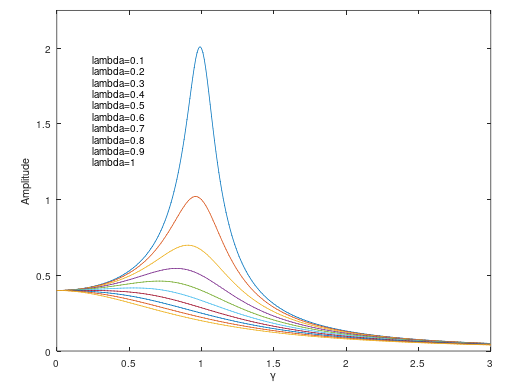
\includegraphics[width=10cm]{chapter_05_paragraph_26}
		\caption{Amplitude de la solution (\ref{EQ:26_3}) avec des valeurs du c{\oe}fficient de frottement compris entre 0.01 et 1.0 et $\omega_{0} = 1$, $f = 2$ et $m = 5$}\label{FIG:5_26}
	\end{center}
\end{figure}

De fait, la partie r\'{e}elle de la solution $x = Be^{i\gamma\mathrm{t}} = be^{i\gamma\mathrm{t} + \delta}$ est l'int\'{e}grale particuli\`{e}re de l'\'{e}quation (\ref{EQ:26_1}), i.e. $\cos(\gamma\mathrm{t} + \delta)$ alors que la solution de l'\'{e}quation sans second membre est celle obtenue en (\ref{EQ:25_4}), i.e. $ae^{-\lambda\mathrm{t}}\cos(\omega\mathrm{t} + \alpha)$ avec $\omega = \sqrt{\omega_{0}^{2} - \lambda^{2}}$dans le cas o\`{u} $\lambda < \omega_{0}$. Ainsi la solution est :
\be
	x = ae^{-\lambda\mathrm{t}}\cos(\omega\mathrm{t} + \alpha) + b\cos(\gamma\mathrm{t} + \delta) \label{EQ:26_4}
\ee
avec $\omega = \sqrt{\omega_{0}^{2} - \lambda^{2}}$. Elle devient après un temps suffisamment long pour que le permier terme tende vers 0 :
\be
	x = b\cos(\gamma\mathrm{t} + \delta) \label{EQ:26_5}
\ee
Lorsque les valeurs de $\gamma$ et $\omega_{0}$ se rapprochent, l'amplitude des oscillations forc\'{e}es obtenues dans la relation (\ref{EQ:26_3}) augmente mais ne tend pas vers l'infini comme cela est le cas en l'absence de frottement, voir la relation (\ref{EQ:22_5}). Quelque soit la valeur de l'amplitude $f$ de la force ext\'{e}rieure, l'amplitude de l'oscillation $b$ est maximale si et seulement si la quantit\'{e} $(\omega_{0}^{2} - \gamma^{2})^{2} + 4\lambda^{2}\gamma^{2}$ est minimale, i.e. :
\bea
	\dfrac{\partial\left((\omega_{0}^{2} - \gamma^{2})^{2} + 4\lambda^{2}\gamma^{2}\right)}{\partial\gamma^{2}} & = & 0 \nonumber \\
	\Leftrightarrow 2\gamma^{2} + 4\lambda^{2} - 2\omega_{0}^{2} & = & 0 \nonumber \\
	\Leftrightarrow \gamma = \sqrt{\omega_{0}^{2} - 2\lambda^{2}} \nonumber
\eea
ce qui permet de remarquer que dans la cas o\`{u} $\lambda \ll \omega_{0}$ alors la valeur de $\gamma$ ne diff\`{e}re de celle de $\omega_{0}$ que par un infiniment petit du second ordre.

\subsection{Au voisinage de la r\'{e}sonance}

Posons dans ce cas $\gamma = \omega_{0} + \epsilon$ avec $\epsilon$ petit devant $\omega_{0}$ et en consid\'{e}rant $\lambda \ll \omega_{0}$ alors 
\benn
	\begin{cases}
		\gamma^{2} - \omega_{0}^{2} = (\gamma - \omega_{0})(\gamma + \omega_{0}) = \epsilon(2\omega_{0} + \epsilon) = 2\omega_{0}\epsilon + \epsilon^{2} \approx 2\omega_{0}\epsilon \\
		2\lambda\gamma i = 2\lambda(\omega_{0} + \epsilon)i \approx 2\lambda\omega_{0}i
	\end{cases}
\eenn
de sorte que l'\'{e}quation (\ref{EQ:26_2}) devient :
\be
	B = - \dfrac{f}{2m\omega_{0}(\epsilon - 2\lambda i} \label{EQ:26_6}
\ee
et l'\'{e}quation (\ref{EQ:26_3}) :
\be
	\begin{cases}
		b = \dfrac{f}{m\sqrt{4\omega_{0}^{2}\epsilon^{2} + 4\lambda^{2}\omega_{0}^{2}}} = \dfrac{f}{2m\omega_{0}\sqrt{\epsilon^{2} + \lambda^{2}}} \\
		\tan\delta = \dfrac{2\lambda\gamma}{\gamma^{2} - \omega_{0}^{2}} = \dfrac{2\lambda\omega_{0}}{2\omega_{0}\epsilon} = \dfrac{\lambda}{\epsilon} \label{EQ:26_7}
	\end{cases}
\ee
Par d\'{e}finition, $\epsilon = \gamma - \omega_{0}$ soit :
\benn
	\tan\delta = \dfrac{\lambda}{\gamma - \omega_{0}} \Rightarrow \dfrac{\partial\tan\delta}{\partial\gamma} = -\dfrac{\lambda}{2(\gamma - \omega_{0})^{2}}
\eenn
ainsi, quelque soit la valeur de $\gamma$, la d\'{e}riv\'{e}e pr\'{e}c\'{e}dente, qui repr\'{e}sente la diff\'{e}rence de phase par rapport \`{a} la fr\'{e}quence de la force ext\`{e}rieure, est toujours n\'{e}gative. Ainsi, l'oscillation du syst\`{e}me retarde sur la force ext\`{e}rieure.

Loin de la r\'{e}sonance, i.e. en reprenant le r\'{e}sultat de (\ref{EQ:26_3}) et en continuant de supposer $\lambda \ll \omega_{0}$, nous avons :
\benn
	\begin{cases}
		\gamma < \omega_{0}\text{, }\tan\delta < 0\text{ et tend vers 0 quand }\gamma\rightarrow\infty \Rightarrow \delta \rightarrow 0\text{, i.e. cos > 0 et sin < 0} \\
		\gamma > \omega_{0}\text{, }\tan\delta > 0\text{ et tend vers 0 quand }\gamma\rightarrow\infty \Rightarrow \delta \rightarrow -\pi\text{, i.e. cos < 0 et sin < 0} \nonumber \\
	\end{cases}
\eenn
Alors qu'\`{a} la r\'{e}sonance, soit $\gamma = \omega_{0}$, nous avons $\delta = \frac{\pi}{2}$. De plus, la variation de la phase $\delta$ de l'oscillation forc\'{e}e entre $-\pi$ et $0$ s'op\`{e}re sur une largeur de fr\'{e}quence $\sim \lambda$ \'{e}troite puique nous avons toujours $\lambda \ll \omega_{0}$. En l'absence de frottement, $\lambda = 0$, le passage de $-\pi$ \`{a} $0$ pour la phase $\delta$ est un saut de valeur $\pi$ et indique que le frottement, finalement, \'{e}tale ce saut.

\subsection{\'{E}nergie}

Une fois le mouvement stabilis\'{e}, l'oscillation est r\'{e}gie par l'\'{e}quation (\ref{EQ:26_5}) et, de facto, l'\'{e}nergie du syst\`{e}me ne varie pas. Ainsi, l'\'{e}nergie absorb\'{e}e aux d\'{e}pens de la force ext\'{e}rieure est dissip\'{e}e par les frottements.

Si $I(\gamma)$ est la quanti\'{e} d'\'{e}nergie dissip\'{e}e en moyenne par unit\'{e} de temps et en fonction de la fr\'{e}quence de la force ext\'{e}rieure, alors l'\'{e}quation (\ref{EQ:25_13}) s'applique et donne :
\benn
	\dfrac{\mathrm{d}E}{\mathrm{t}} = -2F \Rightarrow \dfrac{\Delta E}{\Delta\mathrm{r}} = 2\overline{F} = I(\Gamma)
\eenn
avec $\overline{F}$ la valeur moyenne sur la p\'{e}riode d'une oscillation de la fonction de dissipation, voir (\ref{EQ:25_11}). Pour un unique degr\'{e} de libert\'{e}, cetter derni\`{e}re relation donne $F = \frac{\alpha}{2}\dot{x}^{\,2}$. En comparant les \'{e}quations (\ref{EQ:26_1}) et (\ref{EQ:25_14}) avec $(i,j) = (1,1)$, nous posons la relation $m\ddot{x} + kx + \alpha\dot{x} = m\ddot{x} + 2\lambda\dot{x} + \omega_{0}^{2}x$ qui est vraie si et seulement si  $\alpha = 2\lambda m$, impliquant que $F = \lambda m\dot{x}^{\,2}$.

Puisque le mouvement est stabilis\'{e}, l'\'{e}quation (\ref{EQ:26_5}) est exploitable et permet d'\'{e}crire :
\benn
	F = \lambda mb^{2}\gamma^{2}\sin^{2}(\gamma\mathrm{t} + \delta)
\eenn
Or sur une p\'{e}riode d'oscillation, $\langle\sin^{2}\rangle = 1/2$ donc :
\be
	I(\gamma) = \lambda mb^{2}\gamma^{2} \label{EQ:26_8}
\ee
Au voisinage de la r\'{e}sonance, $b$ est donn\'{e} par la relation (\ref{EQ:26_7}) et alors, $I(\gamma)$ devient plut\^{o}t $I(\epsilon)$ tel que :
\bea
	I(\epsilon) & = & \dfrac{\lambda mf^{2}}{4m^{2}\omega_{0}^{2}(\epsilon^{2} + \lambda^{2})}(\omega_{0} + \epsilon)^{2} = \dfrac{\lambda f^{2}}{4m(\epsilon^{2} + \lambda^{2})}\left(1 + \dfrac{\epsilon}{\omega_{0}}\right)^{2} \nonumber \\
	\Leftrightarrow I(\epsilon) & = & \dfrac{f^{2}\lambda}{4m(\epsilon^{2} + \lambda^{2})}\text{ car }\epsilon \ll \omega_{0} \label{EQ:26_9}
\eea
Cette forme de relation entre \'{e}nergie dissip\'{e}e, absorb\'{e}e, et la fr\'{e}quence $\epsilon$ est appel\'{e}e \emph{dispersive}. La valeur maximale de $I$ est atteinte quand $\epsilon$ vaut mieux et elle est de :
\benn
	I(0) = \dfrac{f^{2}}{4m\lambda}
\eenn
De m\^{e}me, la demi-largueur de la courbe, i.e. la largeur à demi-hauteur, se d\'{e}duit de l'\'{e}quation suivante :
\benn
	I(\epsilon) = \frac{I(0)}{2} \Leftrightarrow \dfrac{f^{2}\lambda}{4m(\epsilon^{2} + \lambda^{2})} = \dfrac{f^{2}}{8m\lambda} \Leftrightarrow 2\lambda^{2} = \epsilon^{2} + \lambda^{2} \Leftrightarrow \epsilon = \pm \lambda
\eenn
Ainsi, si le c{\oe}fficient d'ammortissement $\lambda$ diminue, alors la hauteur de la courbe de r\'{e}sonance devient plus importante mais sa demi-largeur diminue. D\'{e}montrons que la surface sous $I(\gamma)$ est invariable par rapport au c{\oe}fficient d'ammortissement $\lambda$.

Comme $\gamma = \omega_{0} + \epsilon$, alors $\mathrm{d}\gamma = \mathrm{d}\epsilon$. Cela permet d'\'{e}crire :
\benn
	\int_{0}^{+\infty}I(\gamma)\mathrm{d}\gamma = \int_{-\omega_{0}}^{+\infty}I(\epsilon)\mathrm{d}\epsilon
\eenn
Or $I(\epsilon) \propto \epsilon^{-2}$ donc $I(\epsilon)$ d\'{e}croit tr\`{e}s rapidement quant $\lvert\epsilon\rvert$ augmente. Par cons\'{e}quent :
\bea
	\int_{-\omega_{0}}^{+\infty}I(\epsilon)\mathrm{d}\epsilon & \approx & \int_{-\infty}^{+\infty}I(\epsilon)\mathrm{d}\epsilon = \dfrac{f^{2}\lambda}{4m}\int_{-\infty}^{+\infty}\dfrac{\mathrm{d}\epsilon}{\epsilon^{2} + \lambda^{2}} \nonumber \\
	& = & \dfrac{f^{2}\lambda}{4m}\int_{-\infty}^{+\infty}\dfrac{\lambda\mathrm{d}\epsilon/\lambda}{\lambda^{2}((\epsilon/\lambda)^{2} + 1} = \dfrac{f^{2}}{4m}\int_{-\infty}^{+\infty}\dfrac{\mathrm{d}X}{(1 + X^{2})} = \dfrac{f^{2}}{4m}\left[\arctan\right]_{-\infty}^{+\infty} \nonumber
\eea
Et enfin, nous pouvons \'{e}crire :
\be
	\int_{-\infty}^{+\infty}I(\epsilon)\mathrm{d}\epsilon = \dfrac{f^{2}\pi}{4m} \label{EQ:26_10}
\ee
permettant de conclure que la surface sous $I(\epsilon)$ ne d\'{e}pend du c{\oe}fficient d'ammortissement du syst\`{e}me.

\section{R\'{e}sonance param\'{e}trique}